\subsubsection{Background and motivation}

The procedure to infer a single global Environment and Gene Regulatory
Influence Network (EGRIN) model from genome-wide data was described
previously \cite{Bonneau2007,Bonneau2006,Reiss2006n}. In short, the
two-step procedure involves running \cm~once to obtain a single set of $\sim 300$
biclusters of genes. Genes in these biclusters have tight co-expression 
over a subset of the measured conditions (usually
about half), are supported by common putative
\textit{cis}-regulatory motif(s) in their promoters (gene regulatory elements, GREs), 
and are often substantiated by high connectivity in functional association networks. 
Next, given a set of ``predictors'' (mRNA expression levels of transcription factors
and/or quantitative values for environmental factors; \eg,
concentrations, growth media, etc.), and the mean expression levels of genes in each bicluster, \nwinf~is run to choose a
parsimonious subset of those predictors that can accurately predict the
expression levels of that bicluster (\ie., those with non-zero
$\beta$ [Eq~\ref{eq:elnet3}]) . Predictors are selected
independently for each bicluster. The combined set of
TF$\rightarrow$bicluster interactions and their associated weights
($\beta$s) give the degree of activation (or repression) predicted.

The \egrine~modeling procedure updates this process by applying 
updated \cm\ and \nwinf\ algorithms (described above)
repeatedly to subsets of the available expression data. The end result
is an ensemble of EGRIN models, each model containing biclusters and
their predicted regulators, tuned to a relatively small subset of the
overall input expression compendium. The experimental subsets were
selected semi-randomly, with available biological information
constraining the selection procedure (\ie., including whole groups of
related experiments when one was randomly selected). For {\it
H. salinarum}, we used manually curated metadata about each experiment
to group related experiments. Since we did not have sufficient metadata 
from the public \textit{E. coli} data set,
 we grouped the conditions based upon individual experiments instead (\eg,
time series). 

The \egrine~inference methodology is an ensemble learning approach,
more specifically a form of bootstrap
aggregation \cite{Breiman96baggingpredictors}, or sub-bagging.
Advantages of sub-bagging include simplicity (\ie, basic model
averaging), reduced model variance
compared to individual runs \cite{Buhlmann2002}, and avoidance of
overfitting \cite{Krogh1997}. The power of ensemble learning
approaches stems from their ability to average out errors in
individual models. For EGRIN models, this feature
helps overcome artifacts due to both experimental and algorithmic
noise. Incorrect classification in a single model that are not the result
of systematic error will re-occur infrequently 
in subsequent runs. Similarly, overfitting is mitigated by training
each individual model on a small subset of the available data. Only consistently re-discovered
relationships are considered significant.

Sub-bagging of experimental conditions further allows the model to
effectively up-weight a restricted set of conditions for each
individual EGRIN model in the ensemble. This forces each EGRIN to
model regulatory behaviors present within a more narrow range of
conditions. As a result, the individual EGRIN models have the
opportunity to discover features that
may distinguish highly related responses or occur in a very limited
number of conditions in the data set (\eg, conditions, genes, GREs). 

To quantify this assumption, we constructed a
separate ensemble of 30 EGRIN models trained on the
complete {\it H. salinarum} data set (\ie, 1,495 conditions; no
sub-setting performed). We asked how often we would discover a GRE
corresponding to the well-characterized anoxic \textit{H. salinarum} TF, Bat. 
Given frequent detection of the Bat GRE in our full
ensemble, we expected to detect $\sim 20$ instances of the Bat GRE in the new ensemble
(\ie, motifs similar to GRE \#22;
Figure \ref{fig:gre_clustering} \cite{Baliga2001}). Surprisingly, we did
not detect a single GRE matching Bat when
all conditions were used for training (data not shown). 
This is likely because the anoxic conditions
in which Bat is active represents only
a small portion of the entire data set.

Ensemble-based approaches are being used more frequently in biological
data analyses, including random forests (\ie, bags of decision trees)
\cite{breiman2001}, and the recently-published DREAM5 community 
ensemble of regulatory network predictions \cite{Marbach2012}, which
we used as a benchmark in this manuscript to evaluate \egrine
predictions for \eco. Moreover, in principle, our approach is similar
to the stochastic \tmsamp{LeMoNe} algorithm \cite{Joshi2009}, which
uses Gibbs sampling to learn ensembles of regulatory modules from gene
expression data. \egrine~is distinguished from \tmsamp{LeMoNe} and
similar algorithms by its ability to predict transcriptional control
mechanisms (\ie, GREs) and the conditions in which they operate, both
globally and within individual gene promoters.

To construct and mine the \egrine~ensemble we utilized additional
model aggregation and compilation procedures, including (1) motif
clustering \cite{vanDongen2012} and scanning \cite{Bailey1998}
(Section \ref{section:gres}); (2) gene co-regulation network
construction and backbone extraction \cite{Serrano2009}
(Section \ref{section:gBg}); and (3) network community
detection \cite{Ahn2010} (Section \ref{section:linkcommunity}). These
methods were used to identify GREs and their genome-wide locations,
gene-gene co-regulatory associations, and corems, respectively. Each
of these procedures is described in more detail below. A comprehensive
workflow is provided in Figure \ref{fig:workflow}.

\begin{figure}[hp]
\centering
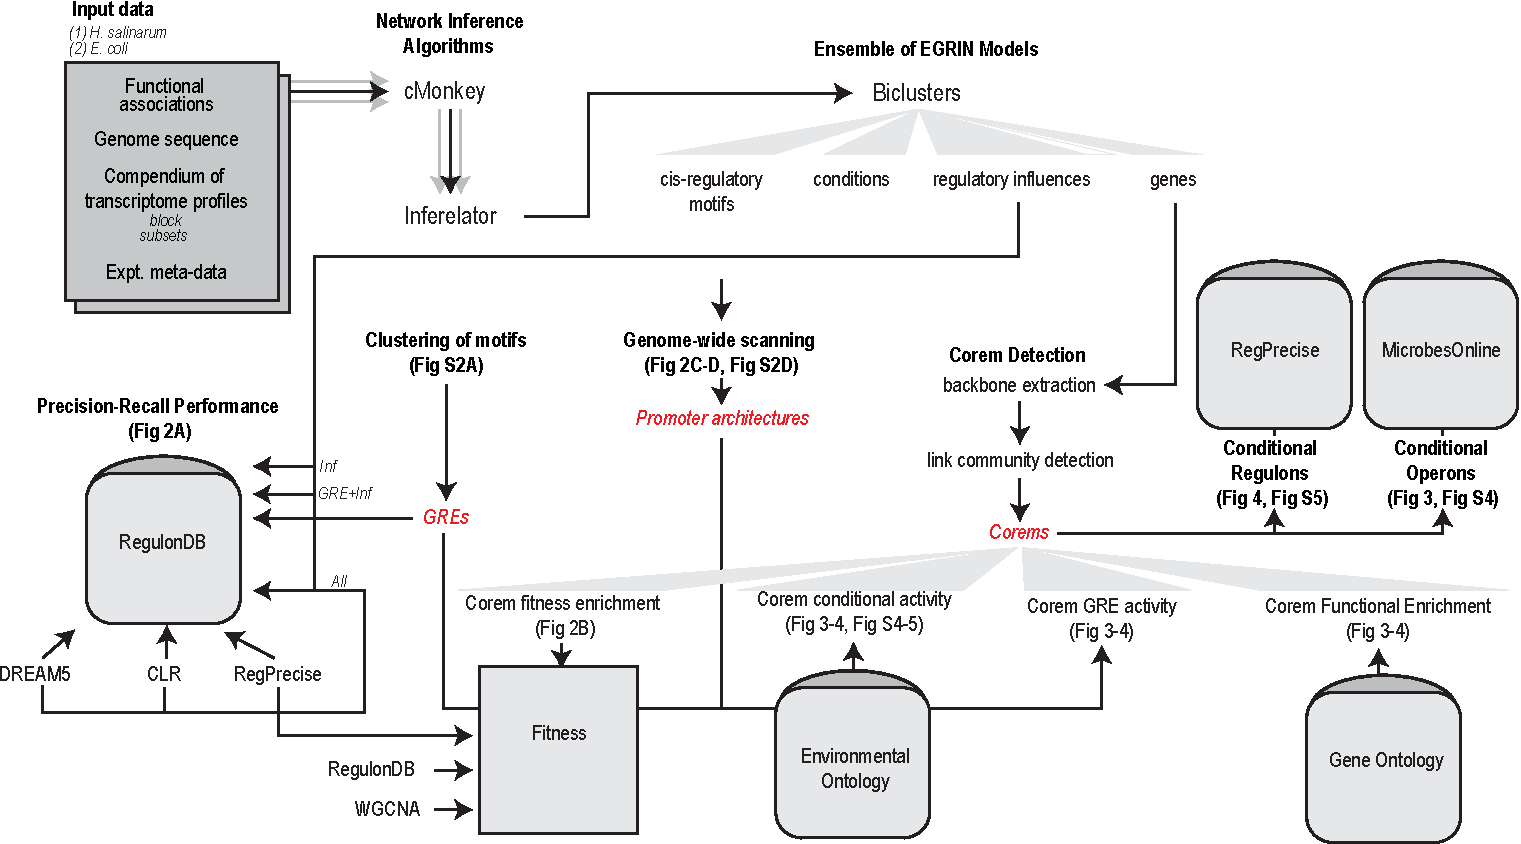
\includegraphics[width=\linewidth]{figures/workflow.pdf}
%\epsfig{file=figures/e1.eps,width=0.95\linewidth}
%\vspace{5in}
\caption[Detailed workflow for \egrine~inference procedure]{
{\bf Detailed workflow for \egrine~inference procedure.} Data input,
processing and analysis to construct \egrine~model for {\it
H. salinarum} and {\it E. coli}, and predictions
generated. Predictions highlighted in individual figures are noted.}
\label{fig:workflow}
\end{figure}

%\subsubsection{Statistical mining of the relationships in the ensemble}
\subsubsection{``Ensemble of EGRINs'': generation and statistical mining}

\egrine~model construction and analysis was performed using
primarily the \tmsamp{R} statistical analysis environment, with add-on
packages \tmsamp{data.table} and \tmsamp{filehash} for off-line
storage (maintaining all information in memory was impossible for our
large ensembles). Once the full set of \cm\ and \nwinf\ runs were
completed and stored, a round of post-processing was performed to
agglomerate all results into a single ad-hoc database for storage and
query. The following relationships could be queried to identify
significant associations between biological entities described in the
model:

\begin{tabular}{|l|l|l|r|} 
\hline
Entity$_1$        & Entity$_2$         & Relationship  & Associated info. \\ \hline
Bicluster         & Gene               & Contains      & - \\
Bicluster         & Condition          & Contains      & - \\
Bicluster         & Motif              & Contains      & Associated genes \\
Regulator         & Bicluster          & Regulates     & Weight \\
Motif             & Motif              & Similar       & $FDR\ q$--value \\
Motif             & Genomic coordinate & Overlaps      & $p$-value \\
\hline
\end{tabular}
\\

\noindent These relationships could then be extended to second-degree
relationships, including (these relationships below are by no means
all-inclusive; for brevity we denote $g$, $g_1$, and $g_2$ as separate
genes, $b$ as a bicluster, $m$ as a motif, $r$ as a regulator, and $c$
as an experimental condition):

\begin{enumerate}
\item $g_1$ is co-regulated with $g_2$ if they occur in the same $b$.
\item $g_1$ is co-regulated with $g_2$ under condition $c$ if $g_1$, $g_2$, and $c$ occur in the same $b$.
\item $m$ regulates $g$ if $m$ and $g$ are both observed in the same $b$.
\item $m$ regulates $g$ under condition $c$ if $m$, $g$, and $c$ are all observed in the same $b$.
\item $r$ putatively regulates gene $g$ via $m$ if $r$ is predicted to regulate $b$ which contains both $g$ and $m$.
\end{enumerate}

%% \begin{tabular}{|l|l|l|r|} 
%% \hline
%% Entity$_1$        & Entity$_2$       & Relationship  & Required mapping \\ \hline
%% Gene$_1$          & Gene$_2$         & Co-regulated  & Gene$_1$ and Gene$_2$ in same bicluster \\
%% Gene$_1$          & Gene$_2$         & Co-regulated under condition $C$  & Gene$_1$ and Gene$_2$ in same bicluster \\
%%                   &                  &               & which also contains $C$ \\
%% Gene$_1$          & Motif            & Regulates     & Gene in same bicluster in which Motif was detected \\
%% \hline
%% \end{tabular}

\noindent The frequency with which any of these relationships occurs throughout the
 entire ensemble of EGRIN models could subsequently be counted by
 querying the database, and a $p$-value describing the significance of
 the frequency computed via the cumulative hypergeometric
 distribution. $p$-values were then converted to false discovery rate
 $q$-values using the Benjamini–Hochberg procedure.  We use this
basic procedure to identify conditions associated with GRE influence,
and GREs associated with gene co-regulation, as we describe below.

%% Statistical associations between any entity in the \egrine~ensemble
%% (\ie, genes, GREs, conditions, TFs; see Figure~1) can be evaluated
%% using the hypergeometric test for statistical enrichment.

\subsubsection{Clustering of cis-regulatory motifs to identify GREs}
\label{section:gres}

Each \cm~ bicluster contains at least one {\it de novo} \MEME -
detected \cite{Bailey1998} {\it cis}-regulatory motif. These motifs
are used by \cm~ to guide bicluster optimization (in addition to other
scoring metrics). There were 86,167 and 269,770 motifs detected across
the entire ensemble for {\it E. coli} and {\it H. salinarum},
respectively. Each motif was represented in the model as a
position-specific scoring matrix (PSSM). To determine which of these
motifs represented \textit{bona fide} GREs (as opposed to false positives), we
computed pairwise similarities between all motifs using \tmsamp{Tomtom} 
\cite{Gupta2007} (Euclidean distance metric; minimum overlap of 6 nt) 
and clustered the most highly similar PSSM pairs
using \tmsamp{mcl} \cite{vanDongen2012}. 

The \tmsamp{Tomtom} motif
similarity $p$-value threshold and the \tmsamp{mcl} inflation
parameter ($I$) were selected to (1) maximize the density (unweighted)
of edges between PSSMs inside clusters relative to the edges between
clusters, and (2) ensure that the \tmsamp{mcl} ``jury pruning
synopsis'' was at least 80 (out of 100). Criterion (1) aims to
find a clustering that is as inclusive as possible, while minimizing
over-clustering, while (2) is a built-in mcl metric that evaluates the
quality of the clusters resulting from the user-selected pruning
strategy ($I$). More specifically for criterion (1), we chose the
clustering parameters (\tmsamp{mcl} inflation parameter
$I$, \tmsamp{Tomtom} $p$-value cutoff $p_c$) which maximize:

\begin{equation}
\label{eq:motif:clust}
\left( I, p_c\right) = \arg \max \left\{ \sum_{I=1}^N \sum_{i=1}^{n_I} \frac{ \sum_{j=1}^{n_I} \delta_{ij} }
                            { \sum_{J=1}^N \sum_{k=1}^{n_J} \delta_{ik} } \right\},
\end{equation}

\noindent where $N$ is the total number of motif clusters for a given set of
parameters, $\delta_{ij}$ indicates a significant similarity (subject
to the given $p$-value threshold) the between PSSMs $i$ and $j$ within
motif cluster $I$ (which contains a total of $n_I$ PSSMs), and
$\delta_{ij}$ indicates a significant similarity between PSSM $i$ in
motif cluster $I$ and PSSM $j$ in motif cluster $J$. The final
parameters that maximized expression~\ref{eq:motif:clust} and
resulted in an \tmsamp{mcl} ``jury pruning synopsis'' of at least 80
were different for the two \egrine~models: $p_c = 10^{-6}$
and \tmsamp{mcl} $I = 4.5$ for the {\it H. salinarum} ensemble and
$p_c = 10^{-5}$ and \tmsamp{mcl} $I = 1.5$ for the {\it E. coli}
ensemble.

We did not filter the motifs by $E$-value or other intrinsic motif
quality metrics; rather, we enforced a cluster size threshold to ensure
that GREs were re-detected consistently. Clusters containing at least
10 PSSMs were considered GREs. This criterion resulted in 
135 GREs for {\it H. salinarum}
(representing 27,991 PSSMs, Table E2) and 337 for {\it E. coli}
(representing 12,773 PSSMs, Table E3). Finally, we computed a
``combined PSSM'' for each GRE as the unweighted mean of aligned PSSMs
within each cluster. This
combined PSSM could be visualized as a motif logo identically to
standard motif PSSMs.

The motif clustering procedure is summarized in Figure \ref{fig:gre_clustering}. 

\begin{figure}[hp]
\centering
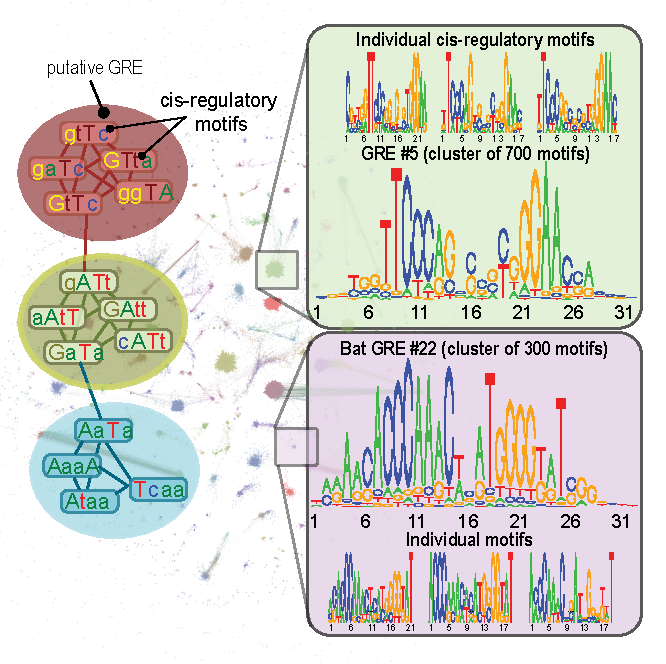
\includegraphics[width=0.8\linewidth]{figures/gre_clustering.pdf}
%\epsfig{file=figures/e2.eps,width=0.8\linewidth}
%\vspace{5in}
\caption[Motif clustering and GRE identification]{\textbf{Motif clustering and GRE identification.} (Left) A schematic of the approach used to align and cluster individually detected motifs to define GREs. In this example, similar motifs were aligned and clustered into three GREs using Tomtom and mcl (Details in Methods and Supplementary Methods). (Center) The {\it H. salinarum} network of aligned and clustered motifs. (Right) Two {\it H. salinarum} GREs discovered by this method. The motif logo of each GRE was generated by summing PSSMs of the individual aligned motifs in the cluster, as illustrated by three examples of individual motifs (prior to alignment) for each of the two GREs. Note that relative to the individual motifs, the averaged GRE motif is more palindromic - a hallmark of binding sites for dimeric TFs.}
\label{fig:gre_clustering}
%\vspace{-.1in}
\end{figure}

\subsubsection{Genome-wide scanning of motifs to obtain GRE locations}
\label{section:scanning}

We used motif scanning to discover GRE locations that were missed by
the rigid definition of a promoter in cMonkey (typically -250 to +50
nucleotides surrounding the translation start site). This procedure
was critical for discovering GREs in non-canonical locations, such as
internal to operons. We computed how well each PSSM (described above)
matched every position in the genome
using \tmsamp{MAST} \cite{Bailey1998}, and recorded significant
matches at each genomic location subject to a position $p$-value
threshold of $10^{-5}$. This $p$-value cutoff corresponds to an
expectation of discovering $\sim 20$ sites at random across the
genome. For each GRE, we summed the number of significant matches to
each of the GRE’s PSSMs at each genomic position. These counts were
used to represent GRE composition in promoters (Figures~2-3). In
addition, we used these scanned locations to identify GREs located
predominantly inside coding regions. Since these GREs may be spurious
(\eg, protein sequence motifs or trinucleotide patterns) they were
flagged, although they were not removed from our global analysis.

We compared the genome-wide distribution of GRE locations to annotated
start sites in \textit{H. salinarum}.  We discovered that most GREs
occur in consistent locations with respect to gene start sites.  The
global position of all GREs and select GREs relative to experimentally
determined gene start sites is depicted in
Figure \ref{fig:gre_global_locs_hal}.

\begin{figure}[hp]
\centering
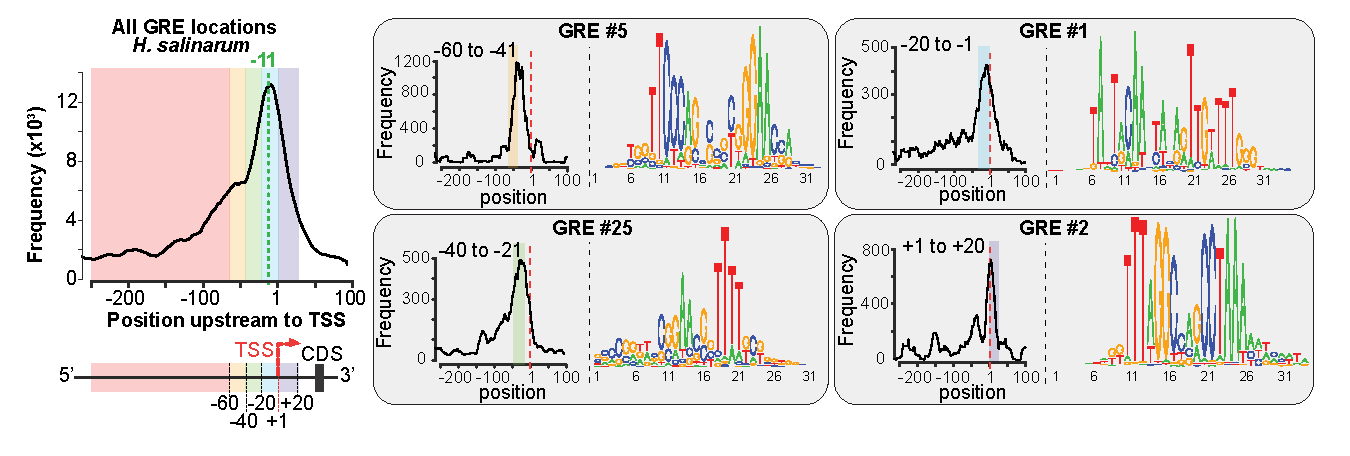
\includegraphics[width=0.95\linewidth]{figures/gre_global_locs_hal.pdf}
\caption[Genome-wide distribution of GREs relative to experimentally mapped transcriptional start sites in \textit{H. salinarum}]{\textbf{Genome-wide distribution of GREs relative to experimentally mapped transcriptional start sites in \textit{H. salinarum}.} (Left) Predicted positions for all GREs in gene promoters upstream of experimentally mapped transcription start sites (TSSs; \cite{Koide2009}) in and (Right) four example elements. Distribution peaks for most GREs occur at characteristic locations. For instance, the location of TATA box-like elements
(GRE \#25) between -21 to -40 nt upstream to TSSs in {\it
H. salinarum} is consistent with the characterized location of basal
elements in archaeal promoters (-25 to 30 nt upstream to TSS). GRE
location enables prediction of putative roles for the cognate TF (\eg
repressor, activator or a basal factor).}
\label{fig:gre_global_locs_hal}
\end{figure}

